\documentclass[twocolumn=on,DIV=calc]{scrartcl}
\usepackage[portuguese]{babel}
\usepackage[colorlinks,allcolors=blue]{hyperref}
\usepackage[utf8]{inputenc}
\usepackage{microtype}
\usepackage[labelsep=period]{caption}
\usepackage{amsmath}
\usepackage{graphicx}
\newcommand{\dpar}[1]{\left(#1\right)}
\newcommand{\un}[1]{\mathrm{#1}}

\DeclareMathOperator{\sen}{sen}
\DeclareMathOperator{\pr}{pr}

\title{Física Geral I: Lista de exercícios 5}

\author{Entregar antes do 4 de julho de 2018}

\date{}

\begin{document}
\maketitle

\paragraph{Instruções}

\begin{itemize}
\item Fazer a questão correspondente ao último algarismo do seu RA. Se
  esse for $0$, faça a questão 10.
\item Além da questão anterior, faça uma outra questão de sua escolha.
\end{itemize}

\paragraph{Questões}


\begin{enumerate}
\item Uma bola, inicialmente em repouso, desliza por um tobogão sem
  atrito de acordo com a figura~\ref{fig:4}. Determine a altura mínima
  $h$ a partir da qual a bola deve ser solta para que ela consiga
  passar por cima do muro de $3\,\un m$ de altura.
  \begin{figure}[ht]
    \centering
    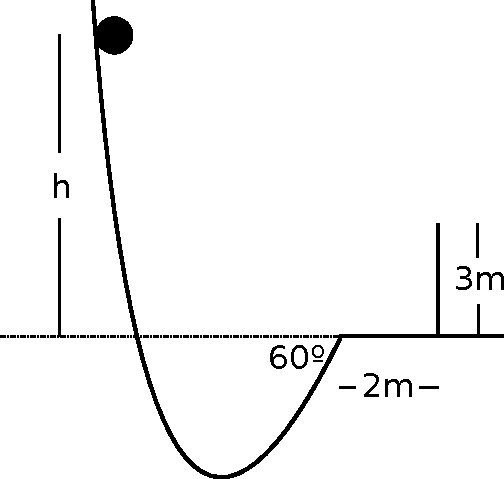
\includegraphics[width=0.4\textwidth,keepaspectratio]{lista5-questao4.pdf}
    \caption{}
    \label{fig:4}
  \end{figure}
\item Uma bola, inicialmente em repouso, é solta desde uma altura
  $h=10\,\un{m}$ e desliza por um tobogão de superfície rugosa de
  acordo com a figura~\ref{fig:4}. Determine o trabalho realizado pela
  força de atrito sobre a bola devido ao tobogão sabendo que a bola
  colide no muro de $3\,\un{m}$ de altura logo de $0{,}4\,\un{s}$ após
  sua saída do tobogão. (Massa da bola: $1\,\un{kg}$).
\item Na figura~\ref{fig:5}, um bloco vai subir uma colina cujo ponto
  mais alto é horizontal. Determine a velocidade mínima com a qual o
  bloco deve subir a colina para que ele não caia no precipício de
  $6\,\un{m}$ de comprimento. (Despreze atritos)
  \begin{figure}[ht]
    \centering
    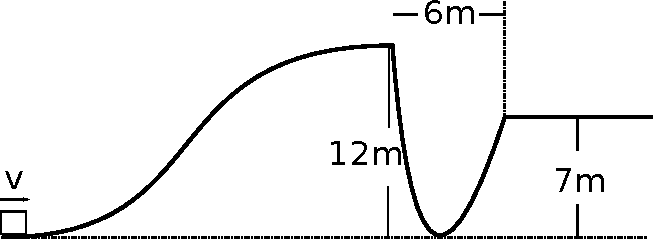
\includegraphics[width=0.45\textwidth,keepaspectratio]{lista5-questao5.pdf}
    \caption{}
    \label{fig:5}
  \end{figure}
\item Uma força de $20\,\un N$ é aplicada sobre um bloco de
  $5\,\un{kg}$, inicialmente em repouso, que pode deslizar por uma
  superfície reta que tem uma parte lisa e outra rugosa (ver
  figura~\ref{fig:3}). (i)~Se a distância entre os pontos $1$ e $2$
  (parte lisa) é de $4\,\un{m}$, determine a velocidade do bloco no
  ponto $2$. (ii)~Se depois do ponto $2$ não se aplica mais a força
  sobre o bloco, determine a distância que ele percorre na parte
  rugosa até se deter sabendo que o coeficiente de atrito cinético
  nessa parte é $\mu_c=0{,}8$.
  \begin{figure}[ht]
    \centering
    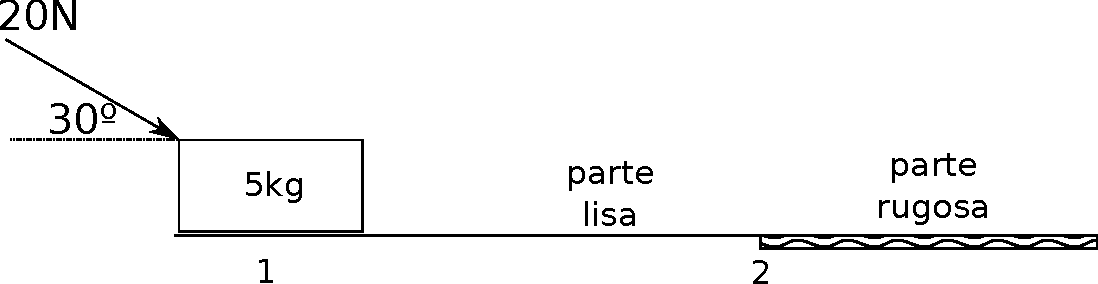
\includegraphics[width=0.45\textwidth,keepaspectratio]{lista5-questao3.pdf}
    \caption{}
    \label{fig:3}
  \end{figure}
\item A figura~\ref{fig:7} mostra um bloco de $5\,\un{kg}$ no ponto
  $1$ que está inicialmente em repouso comprimindo uma mola, cuja
  constante é $k=10\,\un{N}/\un m$. (i) Determine a distância que a
  mola deve ser comprimida, em relação ao seu ponto de equilíbrio,
  para que o bloco consiga andar $10\,\un{m}$ na parte rugosa antes de
  se deter. (Coeficiente de atrito cinético $\mu_c=0{,}6$). Determine
  também a velocidade do bloco no ponto $2$.
  \begin{figure}[ht]
    \centering
    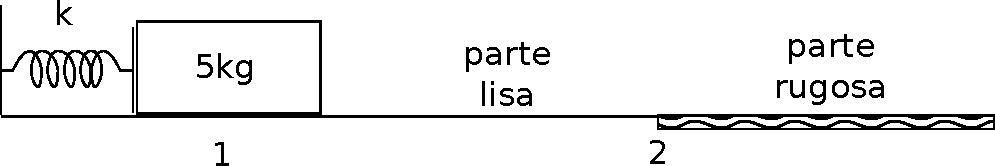
\includegraphics[width=0.45\textwidth,keepaspectratio]{lista5-questao7.pdf}
    \caption{}
    \label{fig:7}
  \end{figure}
\item A figura~\ref{fig:2} mostra uma esfera $A$ sobre uma mesa a qual
  está unida a uma outra esfera $B$ por uma corda que passa por um
  orifício da mesa. A esfera $A$ desliza sem atrito sobre a mesa
  realizando um movimento circular uniforme de raio
  $R=0{,}5\,\un{m}$. Se as massas das esferas são $m_A=0{,}2\,\un{kg}$
  e $m_B=2\,\un{kg}$ e a esfera $B$ está a uma certa altura do chão,
  determine o módulo da velocidade da esfera $A$ para que a esfera $B$
  não caia.
  \begin{figure}[ht]
    \centering
    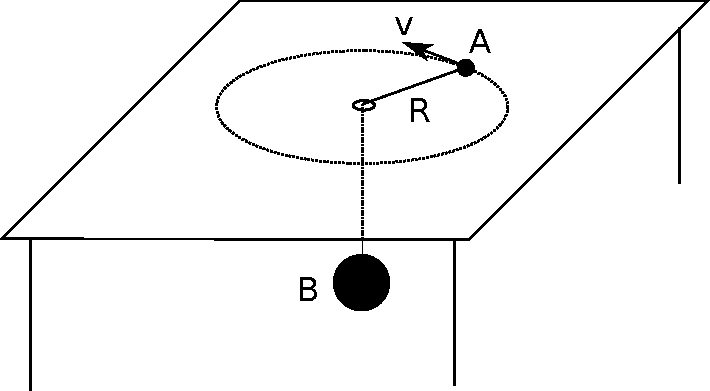
\includegraphics[width=0.45\textwidth,keepaspectratio]{lista5-questao2.pdf}
    \caption{}
    \label{fig:2}
  \end{figure}
\item A figura~\ref{fig:1} mostra um arame em forma de $V$ e um anel
  que pode deslizar por uma das partes do arame sem atrito. Determine
  o valor da velocidade angular constante $\omega$ para que o anel
  permaneça girando a uma altura $h=1\,\un{m}$.
  \begin{figure}[ht]
    \centering
    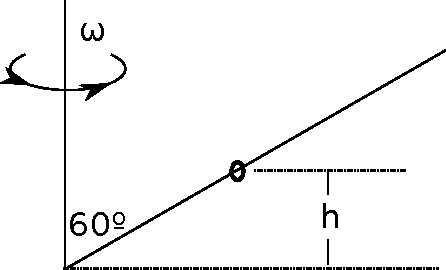
\includegraphics[width=0.4\textwidth,keepaspectratio]{lista5-questao1.pdf}
    \caption{}
    \label{fig:1}
  \end{figure}
\item Um bloco de $2\,\un{kg}$ está inicialmente em repouso no ponto
  mais alto de um plano inclinado (ver figura~\ref{fig:8}). Determine
  a constante da mola $k$ para que o bloco comprima a mola $1\,\un{m}$
  ao se deter. (Despreze atrito)
  \begin{figure}[ht]
    \centering
    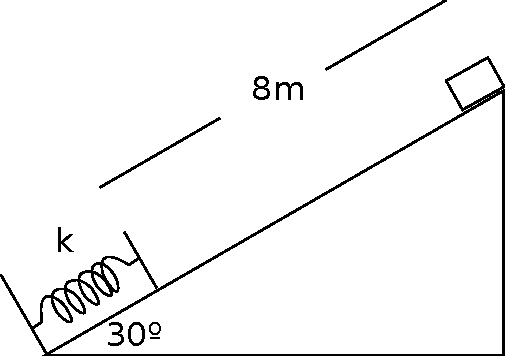
\includegraphics[width=0.45\textwidth,keepaspectratio]{lista5-questao8.pdf}
    \caption{}
    \label{fig:8}
  \end{figure}
\item Na figura~\ref{fig:6}, um bloco de $1\,\un{kg}$ de massa sai do
  ponto $1$ com uma velocidade inicial $v$. Qual deve ser o valor
  mínimo de $v$ para que o bloco consiga chegar no ponto $2$?
  (Coeficiente de atrito cinético da parte rugosa: $\mu_c=0{,}6$).
  \begin{figure}[ht]
    \centering
    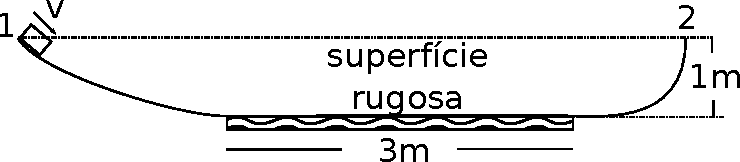
\includegraphics[width=0.45\textwidth,keepaspectratio]{lista5-questao6.pdf}
    \caption{}
    \label{fig:6}
  \end{figure}
\item Usando os dados do exercício anterior, determine a velocidade
  inicial do bloco para que ele se detenha na metade da superfície
  rugosa.
\end{enumerate}
\end{document}